\documentclass{sig-alternate}
%\documentclass{../acm_proc_article-sp}

\usepackage{graphicx}
\usepackage{subfigure}
\usepackage{alltt}

% Define subfloat environment
\newbox\subfigbox % Create a box to hold the subfigure.
\makeatletter
\newenvironment{subfloat}% % Create the new environment.
{\def\caption##1{\gdef\subcapsave{\relax##1}}%
\let\subcapsave=\@empty % Save the subcaption text.
\let\sf@oldlabel=\label
\def\label##1{\xdef\sublabsave{\noexpand\label{##1}}}%
\let\sublabsave\relax % Save the label key.
\setbox\subfigbox\hbox
\bgroup}% % Open the box...
{\egroup % ... close the box and call \subfigure.
\let\label=\sf@oldlabel
\subfigure[\subcapsave]{\box\subfigbox}}%
\makeatother

\special{papersize=8.5in,11in}
\pdfpagewidth=8.5in
\pdfpageheight=11in

\begin{document}

\title{Studying task-level parallelism in sequential programs using Embla}
\numberofauthors{4}
\author{
% 1st. author
\alignauthor
Jonathan Mak\\
       \affaddr{University of Cambridge Computer Laboratory}\\
       \affaddr{15 JJ Thomson Avenue}\\
       \affaddr{Cambridge CB3 0FD, UK}\\
       \email{Jonathan.Mak@cl.cam.ac.uk}
% 2nd. author
\alignauthor
Karl-Filip Fax\'en\\
       \affaddr{Swedish Institute of Computer Science}\\
       \affaddr{Box 1263}\\
       \affaddr{SE-164 29 Kista, Sweden}\\
       \email{kff@sics.se}
\and
% 3rd. author
\alignauthor
Sverker Janson\\
       \affaddr{Swedish Institute of Computer Science}\\
       \affaddr{Box 1263}\\
       \affaddr{SE-164 29 Kista, Sweden}\\
       \email{sverker@sics.se}
% 4th. author
\alignauthor
Alan Mycroft\\
       \affaddr{University of Cambridge Computer Laboratory}\\
       \affaddr{15 JJ Thomson Avenue}\\
       \affaddr{Cambridge CB3 0FD, UK}\\
       \email{Alan.Mycroft@cl.cam.ac.uk}
}
\date{} % do not add a date

\maketitle % optional

\begin{abstract}

Manual parallelization of programs is known to be difficult and error-prone, and there are currently few ways to measure the amount of potential parallelism in the original sequential code.

We present an extension of Embla, a Valgrind-based dependence profiler that links dynamic dependences back to source code, to be used as a tool to estimate, and help programmers realize at a source-code level, inherent task-level parallelism in a sequential program.
Using the popular fork-join model, our tool provides a realistic estimate of potential speed-up for parallelization with frameworks like Cilk or OpenMP 3.0\@.
Estimates can be given for several different parallelization models, varying in programmer effort and capabilities required of the underlying parallel implementation.
Our tool also outputs source-level dependence information to aid the parallelization of programs with lots of inherent parallelism, as well as critical paths to suggest algorithmic rewrites of programs with little.

We validate our claims by running our tool over \emph{serial elisions} of sample Cilk programs and C benchmarks, discovering fresh parallelism in the former, and suggesting parallelism-enhancing algorithmic rewrites in the latter.

\end{abstract}


% \category{D.3.4}{Programming Languages}{Processors}[Compilers]
% \terms{Languages, Measurement}
% \keywords{Limits of parallelism, dynamic dependency graph, spaghetti stack}

\section{Introduction}

Parallel programming is no longer optional.  In order to enjoy continued
performance gains with future generation multicore processors,
application developers must parallelize all software, old and
new
% \cite{TEL95,ONHWC96,KAB03,VIAVAC05}
.  
% For scalable parallel
% performance, program execution must be divided into large numbers of
% independent tasks that can be scheduled on available cores and hardware
% threads by runtime systems.  
While automatic parallelization based on static analysis 
% \cite{KA02}
is sometimes feasible, currently most software requires manual
parallelization.
Since this is a difficult task, there is urgent need for efficient tool support. 
In particular, tools that assist the programmer in understanding the potential 
for parallelization in the code, finding promising parts of the code to parallelize, 
and in validating that the resulting parallel code is correct.

In this paper, we concentrate on the first issue; estimating the potential 
for parallelism in a sequential program. The objective is to construct a tool
which, when given a sequential program and an input, can estimate the 
amount of parallelism that would be available if the program was parallelized
using a language like OpenMP or Cilk. We validate our results against span 
measurements of explicitly parallel Cilk programs.

For explicitly parallel languages, 
such tools are based on the parallelization provided by the programmer, and 
estimates the performance of that particular parallel program. For programs written
in a sequential language, the tool must construct
an {\em estimated parallelization}. This requires two kinds of information:
\begin{itemize}
\item
Information about the program, in particular about the dependencies between 
different parts, since these determine which parallelization is legal (this 
information is also needed to find parallelization opportunities and validating 
correctness).
\item
Information about the parallel execution mechanisms and how these are going
to be integrated into the program, that is, what parallelizing transformations 
will be used.
\end{itemize}
We have implemented a parallelism measurement tool by extending the existing
tool Embla [cite!] (which captures dependence information by an instrumented 
execution of a program) with functionality for simulating the effects of various parallel 
programming models, all based on independent fork-join task parallelism
%\cite{Conway63}
, a framework used in many parallel programming environments.
%\cite{BJKLR96, Lea00, DM98, LF00}.

In traditional studies of parallelism limits, the focus is typically
on hardware support for some model of parallel execution, for instance 
instruction level parallelism in the seminal study by Wall \cite{wall91limits} 
or speculative module level parallelism \cite{warg01limits}. Parameters
such as the amount of hardware resources (buffer space, function
units, \ldots) are then varied. Our focus is rather on explicit
parallelization of the program source code. This leads to a somewhat
different set of parameters to vary and different constraints for
parallelization. For instance, in contrast to e.g. Wall, 
we use control dependence information
in our baseline model since that is typically available for source
level transformations. On the other hand, our baseline model is
static, in the sense that each code section is parallelized in one way
only; this parallelization must be correct in all executions of that
section. This is consistent with source level parallelization, and
special measures have to be taken to lift the restriction (for
instance function cloning, to allow code to be parallelized for some 
call sites and not for others). To fully implement this model, speculative 
execution (dependence speculation) has to be used. Section~\ref{smethod} 
discusses our parallelization models in depth.

We have used our prototype tool to investigate the potential for 
parallelization of three collections of programs; the SPEC CPU 2000 
integer programs, miBench and the example programs distributed with
the Cilk 5.4.6 distribution. While the two first collections contain
sequential programs, the last one is made up of explicitly parallel 
programs in the Cilk 5 language. These have the property that eliding
the parallel construct leaves correct sequential code, and we have run 
our tool on that code as validation of our approach. We can thus contrast 
programs from these different sources as well as show the behaviour of 
the different models, including the effects of control and dependence speculation.
Section~\ref{sresults} reports the results of these experiments.




\begin{figure}
\small
\hrulefill
\[
\begin{minipage}[t]{3cm}
\begin{alltt}
   p();
   q();
   r();
\end{alltt}
\end{minipage}
\begin{minipage}[t]{3cm}
\begin{alltt}
   spawn p();
   q();
   sync;
   r();
\end{alltt}
\end{minipage} 
\]
\hrulefill
\caption{Example of fork-join parallelism.}
\label{fforkjoin}
\end{figure}

Consider the program fragment in
Figure~\ref{fforkjoin} (left):
Suppose that the calls to {\tt p()} and {\tt q()} are independent,
but that the call to {\tt r()} depends on the earlier calls. Then
the call to {\tt p()} can be
executed in parallel with
the call to {\tt q()}, as shown to the right.
Here we assume the availability of a construct {\tt spawn} to start
the call in parallel and {\tt sync} to wait for all {\tt spawn}'d
activities to terminate (cf. Cilk
%\cite{BJKLR96}
).
% As long as {\tt p()} and {\tt q()} are
% independent, the parallel program will produce identical results to
% the sequential version.  Therefore it is sufficient to understand
% (debug, verify, \ldots) the sequential program; everything except
% performance carries over to the parallel version.



\section{Methodology}

The aim of studying task-level parallelism is to separate out instruction-level parallelism, which is already exploited in superscalar and VLIW machines, and coarser-grain parallelism more suited for multiple cores, where threading and communication overheads would nullify gains from fine-grain parallelism.
However, in order to find the limits of task-level parallelism we must first define what a task is.
Consistent with many other studies \cite{Kreaseck00limitsof}, we define a task as either a function call or a loop iteration.
Though such a definition is perhaps restrictive, we feel it is justifiable.
Functions tend to contain a substantial amount of work---it is rare that a function would be defined simply to execute one statement.
As for loops, loop iterations would tend to have close execution times, and should therefore lead to small load imbalance when parallelised.
Also, the use of existing programming constructs means that the task-level parallelism that we discover can be extracted by both programmer and compiler easily.
It is no surprise that popular parallel programming languages such as Cilk \cite{blumofe96cilk} and OpenMP \cite{dagum98openmp} also use function calls and loops as their primary parallel constructs.

The way we calculate potential parallelism is by the construction of a dynamic dependency graph for each function call.
A dynamic dependency graph is a directed acyclic graph $G=(V,E)$ where each node $v\in V$ corresponds to an execution of a line of the program\footnote{Ideally we would like to have each node corresponding to the execution of a statement, but gcc debug information has been inadequate for this.}, and each edge $e\in E$ corresponds to a dependency between two line executions.
Such a dependency means that they cannot be executed in parallel---the source must be completed before the target can begin.
The critical path $CP$ is then defined as the path in $G$ with the largest total cost.
The limit of parallelism for a function call is then defined as the cost of serial execution divided by the length of the critical path, i.e. $\frac{\sum_{v\in V} cost(v)}{\sum_{v\in CP} cost(v)}$.

We now examine the exact dependencies that are considered in our analysis.

\subsection{Data dependencies}
Data dependencies arise when two lines of a program access the same memory location, and at least one of them writes to it.
These can be categorised into three types---true (read-after-write), anti- (write-after-read) and output (write-after-write) dependencies.
In our study we consider data dependencies in two ways---dynamic and static.

\begin{figure}
  \centering
  \begin{verbatim}
    void g1(int *a) {
      ...
      *a = ...; // Writes to *a
    }
  
    void g2(int *b) {
      ... = *b; // Reads from *b
      ...
    }

    int f(int *a, int *b) {
      int x;
      g1(a);
      g2(b);
    }

    int main(int argc, char *argv[]) {
      int x=0, y=1;
      f(&x, &y);
      f(&x, &x);
    }
  \end{verbatim}
  \caption{}
  \label{datadeps}
\end{figure}

When considering dynamic data dependencies, each function call is analysed independently to find its data dependencies.
With static data dependencies, however, the same set of dependencies is used for all calls to the same function.
The difference can be illustrated in the program in figure \ref{datadeps}, where there is a potential dependency between the calls to \texttt{g1} and \texttt{g2} in \texttt{f}.
A model using static data dependencies would place that dependency in all calls to \texttt{f}, while one using dynamic dependencies would only place it in the second call.

\subsection{Control dependencies}
When whether a line is executed is not known until the execution of another, the former line is said to be control dependent on the latter.
In our study we consider three models of control dependencies: Last Executed Branch (LEB), Control Flow Analysis (CFA) and None.

\begin{description}

\item[Last Executed Branch (LEB)]
We make every line dependent on the last executed line that included a branch (i.e. an \texttt{if} conditional or a \texttt{switch}).
This prevents a conditional from being evaluated at the same time of anything that comes after it.
It provides a safe approximation to actual control dependencies but requires no static analysis.

\item[Control Flow Analysis (CFA)]
The LEB model could be over-conservative, as control flow merges are not considered.
That is, in that model a statement coming after an \texttt{if-else} block would still be control dependent on the conditional of that block even though that statement would be executed whichever way the branch went.
To resolve this issue we perform static control flow analysis on the program, by constructing a Control Dependence Graph \cite{ferrante87program} for each function in the program.
The result means we would only enforce a control dependency where it is actually necessary.

\item[None]
Our final model ignores control dependencies completely.
In effect this gives us the limits of parallelism in the presence of control speculation, or in other words how much parallelism is achievable if we can predict which way a branch goes with 100\% accuracy.
Previous studies on branch prediction \cite{smith98study} suggest that even simple and compile-time prediction algorithms can result in high accuracies for many programs, and therefore this model may not actually be so unrealistic.

\end{description}

\subsection{Loops}
As mentioned above, we have defined a task to be either a function call or a loop iteration.
While function calls are easy to recognise, loops are harder to identify during runtime.
Furthermore, care needs to be taken when marking boundaries of a loop iteration.
For instance, if the statement that increments the loop induction variable is included in the task, then there would be no parallelism possible as each task would read from and then update this loop induction variable, resulting in a dependency between each iteration and the next.
In our analysis loop-level parallelism is studied in two ways.

\subsubsection{Line-level parallelism}
So far, because we would like to identify only function-call level parallelism and not instruction-level parallelism, we insert dependencies to the execution of each line from the last executed line that does not contain a function call.
This has the effect of allowing only lines containing function calls to be spawned, meaning leaf functions (those that do not make any function calls) would exhibit no task-level parallelism.
This, however, would also rule out any loop-level parallelism.
Thus one way to consider loop-level parallelism is by not inserting such dependencies, giving us limits on `line-level' parallelism.
The results would then contain loop-level as well as function-level parallelism, but would also include inter-line instruction-level parallelism (intra-line instruction-level parallelism would still be excluded).

\subsubsection{Natural loop identification}
In order to investigate loop-level parallelism without including instruction-level parallelism in the process, we employ an established natural loop identification algorithm \cite{aho86compilers, muchnick97advanced}.
This algorithm works by looking for \emph{back edges} in the Control Flow Graph, and searching for lines in between the two ends of each back edge.
While this does not identify all loops, most straightforward conventional loops would be found.
We would then consider each iteration, excluding the loop exit line (the one most likely to contain a loop induction variable increment), as a task, just as if it was a function call.

\subsection{Spawn hoisting}

\begin{figure}
  \centering
  \begin{subfloat}
    \begin{minipage}{0.6in}
      \begin{verbatim}
int x, y, r=0;

x = fib(n-1);
r = r + x;
y = fib(n-2);
r = r + y;
return r;


      \end{verbatim}
    \end{minipage}%
    \label{orig}
    \caption{Original program}
  \end{subfloat}%
  \qquad
  \begin{subfloat}
    \begin{minipage}{0.9in}
      \begin{verbatim}
int x, y, r=0;

x = spawn fib(n-1);
sync;
r = r + x;
y = spawn fib(n-2);
sync;
r = r + y;
return r;
      \end{verbatim}
    \end{minipage}%
    \label{without}
    \caption{Without spawn hoisting}
  \end{subfloat}%
  \qquad
  \begin{subfloat}
    \begin{minipage}{0.9in}
      \begin{verbatim}
int x, y, r;

x = spawn fib(n-1);
y = spawn fib(n-2);
r=0;
sync;
r = r + x;
r = r + y;
return r;
      \end{verbatim}
    \end{minipage}%
    \label{with}
    \caption{With spawn hoisting}
  \end{subfloat}%
  \caption{An illustration of spawn hoisting on part of a function that calculates a Fibonacci number.}
  \label{spawn}
\end{figure}

Without spawn hoisting, the only parallelism that is possible is by the spawning of certain lines, with no reorderings possible.
It is however sometimes beneficial to pre-emptively spawn a function call as early as other dependencies allow, rather than waiting for control to reach that program point.
This is equivalent to hoisting function calls to their earliest positions.
Figure \ref{spawn} shows a program where spawn hoisting is required to result in any parallelism.

\subsection{Note about `static' dependencies}
Static analysis aims to extract as much information as possible about the runtime behaviour of a program by only looking at the program source.
The problem of getting exact information about how a program might behave is undecidable in general, especially in the area of alias analysis\cite{landi92undecidability}, and consequently dependency analysis also.
As a result, one can only hope for getting a safe but conservative estimate about possible program behaviour.
Nevertheless, there has been a large body of work that attempts to narrow the gap between the conservative approximation and actual behaviour\cite{kennedy02optimizing}, and advances are still being made (e.g. \cite{raza09automatic}).

In our study, rather than including the state-of-the-art static analysis, which will take a great deal of time and effort as well as risk our results being made irrelevant by newer analysis techniques, we have used a program's runtime behaviour as limits of what can be achieved with static analysis.
What this means is that when we consider static dependencies we must run the program twice.
During the first run, we collect data dependencies and control flow for all calls of each function, which are then aggregated into a set of dependencies for each function definition.
These dependencies are then used for each function call in the second run, regardless of which subset of dependencies would actually arise in each function call.

While our approximation to static analysis is unsafe, it provides a limit on what static analysis can do by aggregating over all calls to the same function over the execution of the program.
Of course there may be dependencies in a program that happen not to materialise in the entire execution when given a certain kind of inputs, which our analysis would miss.
However, we would argue that the infrequency of such dependencies if they exist would make them good candidates for thread-level speculation anyway---ignoring them would give us almost the same speed-up as if the dependencies never existed, as roll-backs would only occur occasionally.

\section{Implementation}

\subsection{Computing Dependencies}   \label{snca}

\begin{figure} \small
\hrulefill
\[
\begin{picture}(160,60)(70,15)
\put(120,65){\makebox(60,10)[c]{\it A:\ \tt f}}
\put(150,65){\line(-2,-1){50}}
% \put(150,65){\line( 0,-1){25}}
\put(150,65){\line( 2,-1){50}}
% \put(95,45){\makebox(20,10)[r]{\it 14}}
% \put(150,45){\makebox(20,10)[l]{\it 15}}
% \put(185,45){\makebox(20,10)[l]{\it 16}}
% \put(70,50){\makebox(20,10)[r]{\ldots}}
% \put(210,50){\makebox(20,10)[l]{\ldots}}
\put(170,30){\makebox(60,10)[c]{\it C:\ \tt g2}}
% \put(120,30){\makebox(60,10)[c]{\it C:\ \tt inc}}
\put(70,30){\makebox(60,10)[c]{\it B:\ \tt g1}}
\put(70,15){\makebox(60,10)[cb]{{\tt *a\ =}\ \ldots}}
\put(170,15){\makebox(60,10)[cb]{\ldots\ {\tt =\ *b}}}
\end{picture}
\]
\hrulefill
\caption{Part of the execution tree of the program in Figure~\ref{datadeps}
% edges are annotated with the line number of the corresponding call.
} 
\label{ffextree}
\end{figure}

Embla traces dependencies between individual instructions in the binary
code during program execution. It then maps these dependencies to 
dependencies between pairs of source lines in the same function. The
instructions causing the dependency need not be part of the function 
within which the dependency is reported. For example, in 
Figure~\ref{datadeps} the instructions causing the dependency (which we
will from now on refer to as the {\em endpoints} of the dependency) 
are part of the bodies of {\tt g1} and {\tt g2}, respectively, wheras the dependency 
will be reported as a dependency between the {\em calls to} {\tt g1} and 
{\tt g2} in {\tt f}.

To find source level dependencies, Embla maintains an {\em execution tree} 
that at each moment captures 
the history of execution up to that moment. Every execution tree node 
corresponds to an
individual function call, and the path from the node to the root of the
tree corresponds to the call stack at the moment of the call. For
example, Figure~\ref{ffextree} depicts a fragment of the execution tree
for the program in Figure~\ref{datadeps}, capturing the calls to {\tt g1} 
and {\tt g2} from {\tt f}.

Embla computes the source-level dependencies
from the instruction-level ones using the execution tree as follows. For
every instruction-level dependency, Embla identifies the function calls
where the endpoints occurred (nodes {\it B} and {\it C} for the example
above), and computes the {\em nearest common ancestor} node (NCA) of
those nodes in the execution tree. The NCA corresponds to a function
call with two instructions that are dependent because of
the instruction-level dependency (the calls to {\tt g1} and {\tt g2} in 
{\tt f} in the example).

\newcommand{\tracepile}{trace pile}


Embla uses two main data structures: The {\em \tracepile}, which represents
the execution tree, and the {\em memory table} which maps addresses to tree
nodes corresponding to the last write and subsequent reads of that
location. The \tracepile\ contains the part of the execution tree
corresponding to the part of the instruction trace that has been
seen so far. Each item in the trace pile corresponds to a memory reference 
or a procedure call or return; an execution tree node corresponds to
a subset of the items.

For each item {\tt n}, {\tt n.parent} is the parent node in the
execution tree (there is also other information associated with a
node, such as what source line corresponds to the node).  The NCA is
computed by following the {\tt parent} links, starting at the earlier
of the instructions corresponding to the dependency, until a node
corresponding to an activation record currently on the call stack is
found. This is the NCA since the later instruction in the pair (which
is also the current instruction), and hence all of its ancestors, are
on the stack.

Once a procedure call has returned, we will not distinguish between 
different events in the subtree corresponding to its (completed) 
execution. The NCA computation will simply skip them, following the 
{\tt parent} links until it finds a node on the stack (which will be
the call instruction at the root of this subtree). Thus we can 
periodically compact the \tracepile\ by replacing subtrees
corresponding to completed calls by their root nodes, saving vast amounts
of memory.
After compaction, the \tracepile\ contains the items associated with the
tree nodes corresponding to the stack, with call instruction items
representing entire subtrees.

Embla uses the Valgrind instrumentation infrastructure which emulates
the user mode instruction set architecture. An interesting alternative
would be to sample dependencies using hardware data breakpoints
(Accumem's Virtual Performance Expert uses this approach for cache
profiling, but since single dependencies are much more important than
single cache misses, it is not clear if sampling is suitable for
dependency analysis).

Our examples of profiling
output use C, but
the profiling is done at instruction level, and the result is
mapped to source level using debugging information.



\section{Results} \label{sresults}

\subsection{Parallelism in Cilk programs} \label{sresults:cilk}

\begin{table}
\small
\begin{tabular}{ | l | l | l | }
\hline
Program & Description & Parameters \\
\hline
\textsf{cholesky} & Matrix decomposition & \texttt{size=256}, \texttt{nonzeros=1000} \\
\textsf{cilksort} & Merge sort & \texttt{size=100000} \\
\textsf{fft} & Fourier transform & \texttt{size=512*512} \\
\textsf{fib} & Na\"ive Fibonacci calculation & \texttt{n=30} \\
\textsf{heat} & Differential equation solver & \texttt{nx=ny=512}, \texttt{nt=1} \\ 
\textsf{lu} & Matrix decomposition & \texttt{n=256} \\
\textsf{magic} & Magic squares search & \texttt{n=4} \\
\textsf{matmul} & Matrix multiplication & \texttt{n=128} \\
\textsf{plu} & Matrix decomposition & \texttt{n=128} \\
\textsf{strassen} & Matrix multiplication & \texttt{n=512} \\
\hline
\end{tabular}
\caption{Description and parameters for Cilk 5.4.6 examples used}
\label{cilk-ex}
\end{table}

We begin by presenting the results of analysing example Cilk programs packaged with the 5.4.6 release of Cilk, as described in Table~\ref{cilk-ex}\footnote{We have omitted programs that use the \texttt{inlet}, \texttt{abort} and \texttt{SYNCHED} keywords, as their translation into ordinary C is not straightforward.}.
As examples packaged with a parallel programming environment, these are programs known to have lots of task-level parallelism.
We ran the original programs in Cilk a number of times to obtain a figure for average parallelism as calculated by Cilk's timing infrastructure.
We then translated these programs into semantically equivalent programs in ordinary C simply by stripping the Cilk keywords\footnote{Namely, \texttt{cilk}, \texttt{spawn} and \texttt{sync}.}.
These \emph{serial elisions} of the original programs are then analysed with our extension of Embla under a number of different models.

\begin{figure}
 \centering
 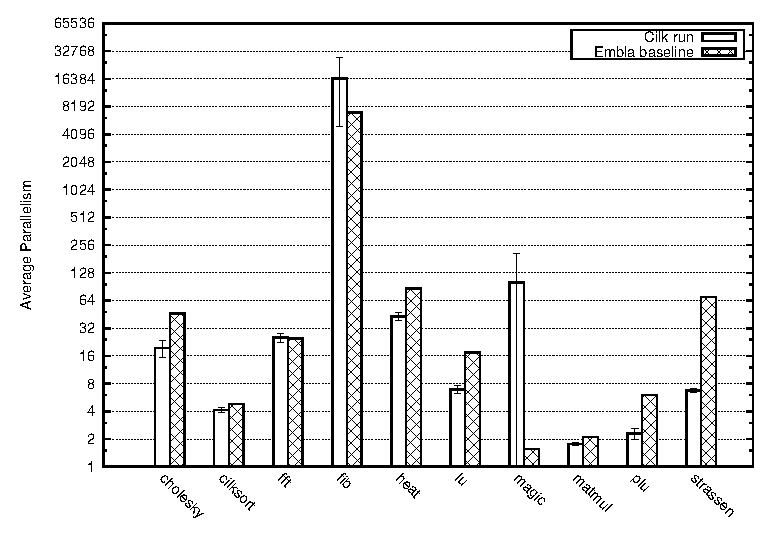
\includegraphics[width=2.9in]{cilk-run}
 \caption{Parallelism of Cilk programs as calculated by Cilk and Embla}
 \label{cilk-run}
\end{figure}

Figure~\ref{cilk-run} compares the parallelism found by Cilk (averaged over 60 runs) to that found by our extension of Embla on their serial elisions.
Our baseline model for this comparison uses aggregated data dependences and control dependences, and considers only function-call-level parallelism without loop parallelization or spawn hoisting---the closest model we have to the one used in Cilk.
The graph shows that our tool is able to find all of the task-level parallelism in most of the original Cilk programs.
The only exceptions are \textsf{fib} and \textsf{magic}, the Cilk parallelism for which appears to vary greatly.
The reason our tool does not find much parallelism in \textsf{magic} compared to the Cilk run is because the Cilk program uses an associative reduction variable in a loop which sums over the results of each iteration, in the form \texttt{for (...) count += spawn(...);}.
Our tool does not currently recognize associative reduction variables, and therefore cannot discover such parallelism.

\begin{figure}[t]
  \begin{center}
  \scriptsize
  \input{cilksort.depgraph}
  \end{center}
  \caption{An extract from \textsf{cilksort} and its corresponding relevant dependences}
  \label{cilksort-depgraph}
\end{figure}

Using aggregated dependences discovered by our tool it is easy to re-insert Cilk keywords into the program to materialize the parallelism discovered.
As an example, Figure~\ref{cilksort-depgraph} shows the aggregated dependences that our tool found for an extract from the \textsf{cilksort} program.
Observe that simply by inserting \texttt{spawn}s in front of function calls, and \texttt{sync}s before the first line that depends on previously spawned tasks, we arrive at the original program.

\begin{figure}
  \begin{center}
  \scriptsize
  \begin{SubFloat}{\label{cilk-sync:without}Original program, showing dependences and best possible parallelization with universal \texttt{sync}s}
    \begin{minipage}{3in}
      \input{lu.depgraph}
    \end{minipage}%
  \end{SubFloat}%
\\
  \begin{SubFloat}{\label{cilk-sync:with}Best possible parallelization if individual \texttt{sync}s were allowed}
    \begin{minipage}{3in}
      \begin{verbatim}
future1 = spawn schur(M00, V00, W00, hnb);
future2 = spawn schur(M01, V00, W01, hnb);
future3 = spawn schur(M10, V10, W00, hnb);
future4 = spawn schur(M11, V10, W01, hnb);

sync future1;
spawn schur(M00, V01, W10, hnb);
sync future2;
spawn schur(M01, V01, W11, hnb);
sync future3;
spawn schur(M10, V11, W10, hnb);
sync future4;
spawn schur(M11, V11, W11, hnb);
      \end{verbatim}
    \end{minipage}%
  \end{SubFloat}%
  \end{center}
  \caption{An example of the greater parallelism caused by individual \texttt{sync}s in an extract from \textsf{lu}.}
  \label{cilk-sync}
\end{figure}


In fact, for a few examples our tool can discover more parallelism than explicitly specified in the original Cilk program.
We found functions called sequentially in \textsf{cholesky}, \textsf{heat} and \textsf{strassen} that could have been spawned.
In addition, we also found C library function calls in \textsf{heat}, \textsf{lu} and \textsf{plu} that cannot be spawned directly in Cilk (as library functions are not defined as spawnable) but can be spawned with the addition of simple wrappers.
The greater parallelism found in \textsf{cholesky}, \textsf{lu} and \textsf{plu} can also be partly attributed to a restriction in Cilk that \texttt{sync}s must join on all tasks spawned rather than any individual task.
If tasks could be synchronized on individually, as illustrated in Figure~\ref{cilk-sync}, then greater parallelism may be found.

We now look more closely at the various models used to examine whether they affect potential parallelism in these programs.

\subsubsection{Data dependences}

\begin{figure}
 \centering
 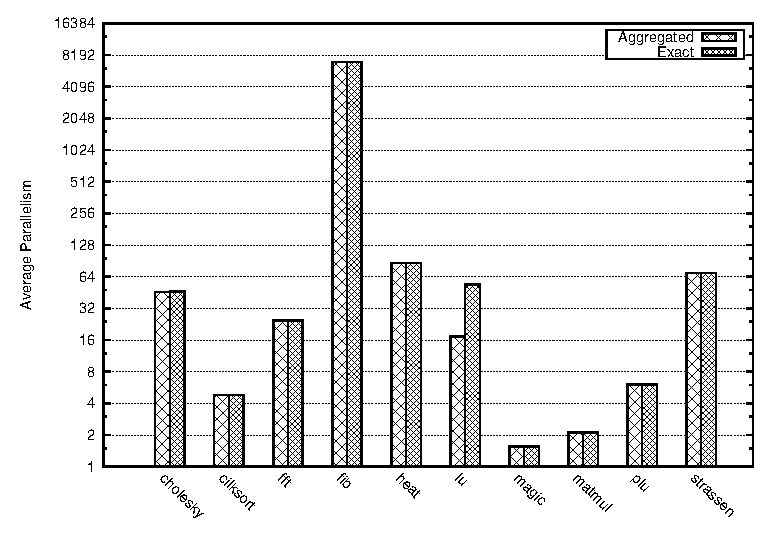
\includegraphics[width=2.9in]{cilk-data}
 \caption{Parallelism of Cilk programs with aggregated and exact data dependences}
 \label{cilk-data}
\end{figure}

Figure~\ref{cilk-data} shows the potential parallelism of the serial elisions of our Cilk examples with aggregated and exact data dependences.
In all programs but \textsf{lu} we see that the difference between the two models is negligible.
This suggests that for most programs most of the potential parallelism is achievable by adding parallel constructs at the source level---runtime techniques such as thread-level speculation would give few performance benefits.

\subsubsection{Control dependences}

%\begin{figure}
% \centering
% 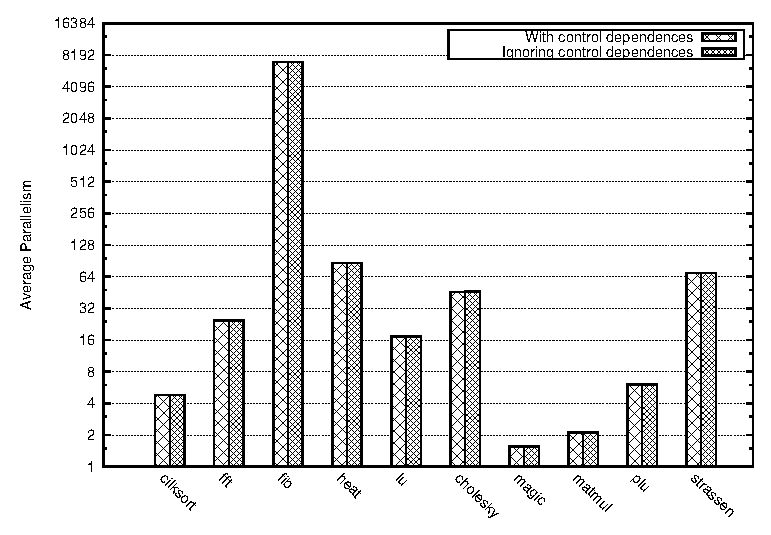
\includegraphics[width=2.9in]{cilk-ctl}
% \caption{Parallelism of Cilk programs with and without control dependences}
% \label{cilk-ctl}
%\end{figure}

%The effects of control speculation are shown in Figure~\ref{cilk-ctl}, which compares the parallelism when control dependences are considered to that when they are ignored.
In all of the programs examined the parallelism is virtually unchanged, when control dependences are ignored, compared to the baseline figures in Figure~\ref{cilk-run}.
This means that for these programs control speculation does not have any effect on available parallelism.
One possible reason for this is that most of these programs are stream-processing-like, with few branches that depend on the data input.
More irregular programs may see greater improvements with control speculation.

\subsubsection{Granularity}

\begin{figure}
 \centering
 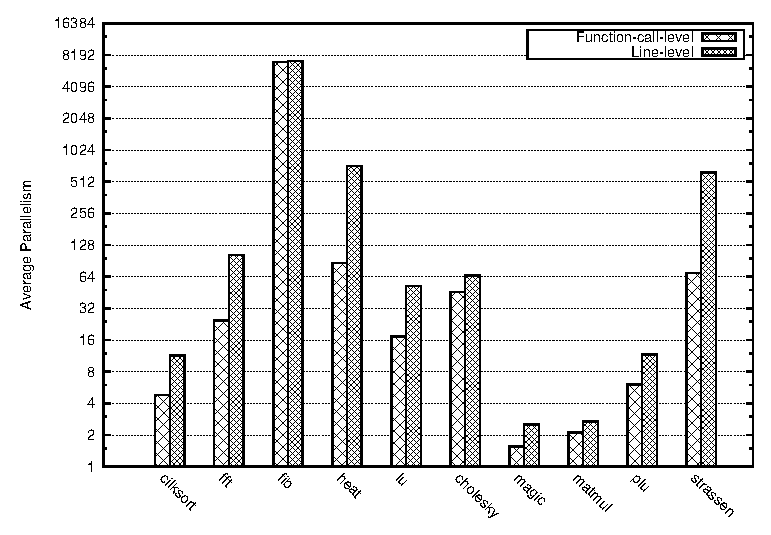
\includegraphics[width=2.9in]{cilk-gran}
 \caption{Parallelism of Cilk programs with different levels of granularity}
 \label{cilk-gran}
\end{figure}

The amount of line-level parallelism in these programs is compared to the amount of task-level parallelism in Figure~\ref{cilk-gran}.
We can see that for most of these programs the amount of line-level parallelism is around twice or more the amount of function-call-level parallelism.
Most of this difference is due to simple statements that perform arithmetic operations inside a function call or loop that can run in parallel.
Each of these operations takes a small number of cycles, which means that it is not viable for each of these to be spawned.
Nevertheless, operations may be grouped and extracted into tasks that are sufficiently large to see performance gains.
We also note that some of this parallelism may well be realized already in existing superscalar or VLIW processors.

\subsubsection{Loops}

\begin{figure}
 \centering
 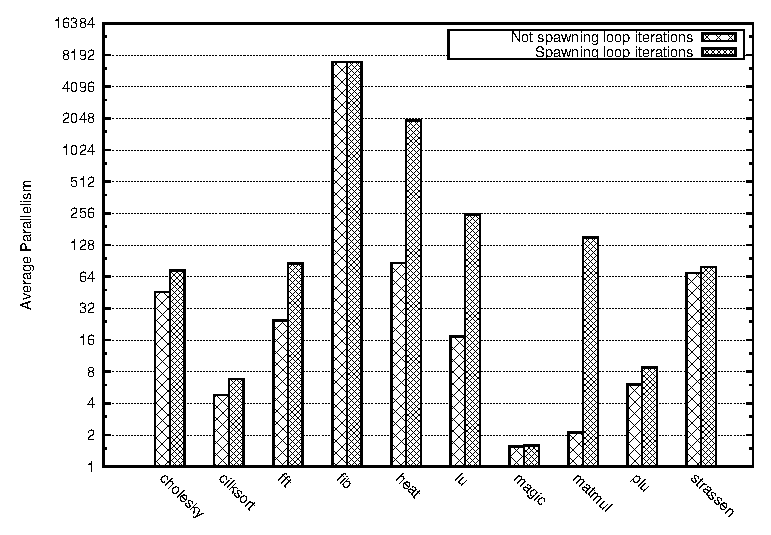
\includegraphics[width=2.9in]{cilk-loop}
 \caption{Parallelism of Cilk programs with and without spawning loop iterations}
 \label{cilk-loop}
\end{figure}

Looking at Figure~\ref{cilk-loop}, which compares the potential parallelism of Cilk programs with and without spawning loop iterations, we can see that the use of parallel for-loops benefit most of the programs considered here.
This is most remarkable in \textsf{matmul}, where there is a 64-fold gain in parallelism when for-loops are parallelized.
We deduce from this that the use of parallel for-loops is an excellent way to express task-level parallelism, in addition to function calls.
Indeed, this justifies the inclusion of parallel for-loops in Cilk++, the commercialized version of Cilk.
Our extension of Embla not only finds the amount of loop-level parallelism in a program, but can be used to easily identify candidate loops for parallelization.
This can simply be done by searching through the dependences output by our tool for dependences between iterations of the loop concerned.
If there are no such dependences, then the loop can be parallelized.

\subsubsection{Spawn hoisting}

%\begin{figure}
% \centering
% 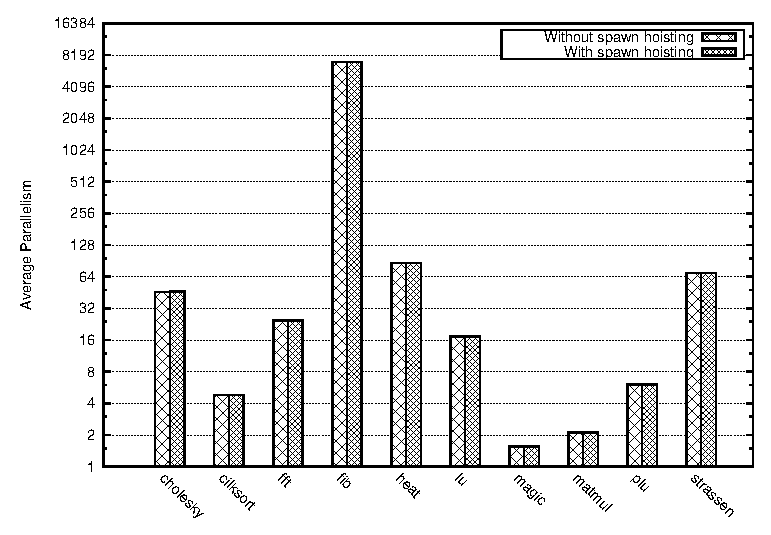
\includegraphics[width=2.9in]{cilk-hoist}
% \caption{Parallelism of Cilk programs with and without spawn hoisting}
% \label{cilk-hoist}
%\end{figure}

%Figure~\ref{cilk-hoist} shows little effect of spawn hoisting on the amount of potential parallelism in the Cilk examples.
With our programs, we find that spawn hoisting has a negligible effect on the amount of potential parallelism in the Cilk examples, as parallelism measurements using spawn hoisting is almost the same as those for the baseline in Figure~\ref{cilk-run}.
This suggests that most function calls are already spawned at the earliest possible point in the program, and there is little further hoisting possible.

\subsection{Parallelism in various benchmarks}

\begin{figure*}
 \centering
 \subfloat[SPEC CPU 2000 integer benchmarks]{
   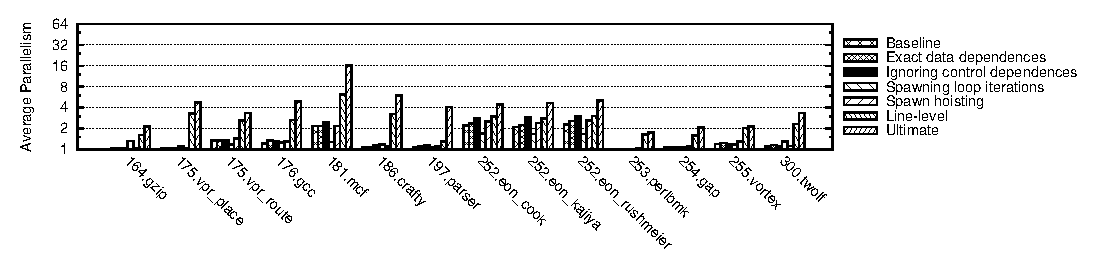
\includegraphics[width=6in]{spec}
 }
 \subfloat[SPEC CPU 2000 floating point benchmarks]{
   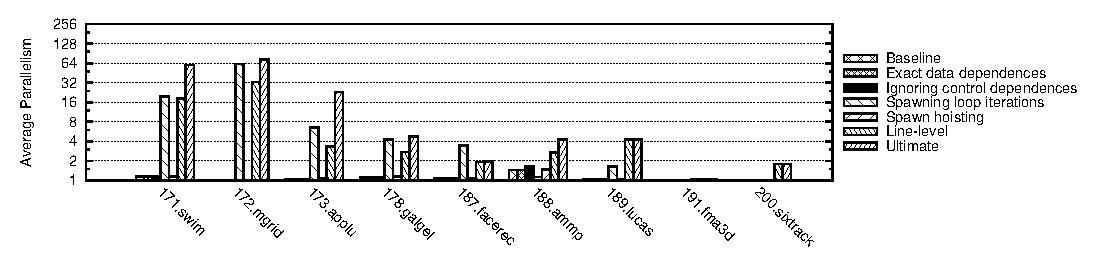
\includegraphics[width=6in]{specfp}
 }
 \subfloat[MiBench]{
   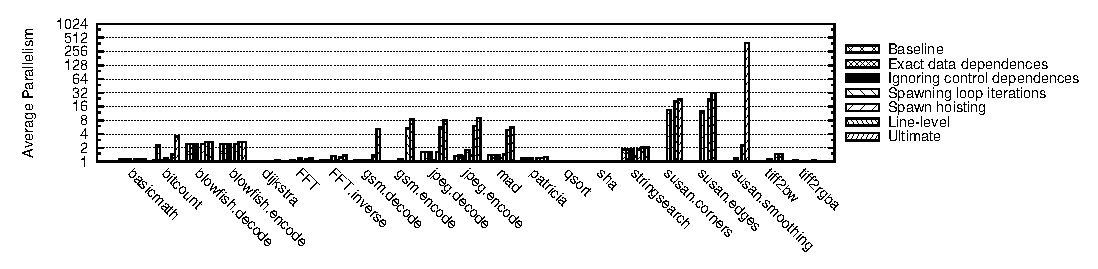
\includegraphics[width=6in]{mb}
 }

\caption{Parallelism of three benchmark suites under various models}
\label{benchmarks}
\end{figure*}

We also ran the same analysis using our tool on some of the benchmark programs in the SPEC CPU 2000 (with the MinneSPEC reduced data input set \cite{KleinOsowski02minnespec}) and MiBench suites, the results of which are displayed in Figure~\ref{benchmarks}.
As before, the baseline model uses aggregated data dependences and control dependences, and considers only function-call-level parallelism without loop parallelization or spawn hoisting.
Each of the other models differs from the baseline by one parameter described in Section~\ref{smethod}, except for \textsf{Ultimate}, which considers line-level parallelism by using exact data dependences, ignoring control dependences and hoisting spawns.
In general, we see that few benchmarks exhibit the level of parallelism seen in the Cilk examples.
In fact, none of these benchmarks exhibit parallelism of over 3 under the baseline model.

There are, however, some benchmarks with a significant amount of loop-level parallelism.
One of them is the MiBench benchmark \textsf{susan}, a program that performs image smoothing, corner detection and edge detection on an image, and is data-parallel---the same computation is performed on each pixel in the image and the results for each pixel are independent of each other.
This is reflected in our results, which show that both \textsf{susan.corners} and \textsf{susan.edges} have potential parallelism of over 12 when loop iterations are spawned.
This is not the case for \textsf{susan.smoothing}, however, as we will explain later.

We note also that for some programs, e.g.\ \textsf{252.eon}, spawning loop iterations actually results in a \emph{lower} level of parallelism.
This is because that while spawning loop iterations allows us to exploit DOALL parallelism, where loop iterations are completely independent from each other and can be executed in parallel, it precludes DOACROSS parallelism or software pipelining, where there are cross-iteration dependences but loop iterations can still partially overlap.
The balance between DOALL and DOACROSS loops would therefore determine whether parallelism rises or falls compared to the baseline.

\subsection{Increasing inherent parallelism by Critical path analysis} \label{sresults:increasing}

Our results suggest that while the example programs from Cilk have lots of inherent task-level parallelism, most general-purpose programs tend to have little and cannot be transformed into highly concurrent programs simply by spawning existing function calls and loops.
Nevertheless, our extension of Embla can output the critical path of each function call, allowing us to examine the bottlenecks that prevent greater parallelism from being realized.
Here we demonstrate the use of critical path information to locate bottlenecks in some of the simpler examples and suggest refactorings or algorithmic changes that would increase inherent parallelism.

\subsubsection{\textsf{sha}}

\begin{figure}
  \begin{center}
    \scriptsize
    \begin{SubFloat}{\label{sha-bottleneck:critpath}Critical path for a call to the \texttt{sha\_stream} function, produced by our tool}
      \begin{minipage}{3in}
        \begin{verbatim}
!sha_driver.c:24(sha.c)=16139892:
200(3460), 198(26614), 198(423934), 198(423934),
198(423934), 198(423934), 198(423934), 198(423934),
198(423934), 198(423934), 198(423934), 198(423934),
198(423934), 198(423934), 198(423934), 198(423934),
198(423934), 198(423934), 198(423934), 198(423934),
198(423934), 198(423934), 198(423934), 198(423934),
198(423934), 198(423934), 198(423934), 198(423934),
198(423934), 198(423934), 198(423934), 198(423934),
198(423934), 198(423934), 198(423934), 198(423934),
198(423934), 198(423934), 198(423934), 198(423934),
197(326)
        \end{verbatim}
      \end{minipage}
    \end{SubFloat}
\\
    \begin{SubFloat}{\label{sha-bottleneck:source}Source for \texttt{sha\_stream} function in \texttt{sha.c}}
      \begin{minipage}{3in}
        \begin{verbatim}
191  void sha_stream(SHA_INFO *sha_info, FILE *fin)
192  {
193      int i;
194      BYTE data[BLOCK_SIZE];
195
196      sha_init(sha_info);
197      while ((i = fread(data, 1, BLOCK_SIZE, fin)) > 0) {
198          sha_update(sha_info, data, i);
199      }
200      sha_final(sha_info);
201  }
        \end{verbatim}
      \end{minipage}
    \end{SubFloat}
  \end{center}
  \caption{Critical Path Analysis of SHA}
  \label{sha-bottleneck}
\end{figure}

\textsf{Sha}, or Secure Hash Algorithm, is a program that computes a 160-bit hash value from the contents of an input file.
Figure~\ref{sha-bottleneck} illustrates part of our analysis into the reason for the lack of inherent parallelism there.
Under the `Line-level' model, our tool reports a critical path of length 16,150,120 instructions out of the total work of 21,968,394 instructions, resulting in a parallelism of 1.36.
From Figure~\ref{sha-bottleneck:critpath}, we see that most of the critical path (16,139,892 instructions) can be attributed to a function call on line 24 in the file \texttt{sha\_driver.c}.
We also see that the critical path consists mainly of dependences between instantiations of line 198 in \texttt{sha.c}, most of which have a cost of 423,934 instructions.
These correspond to calls to \texttt{sha\_update} in the program source (Figure~\ref{sha-bottleneck:source}).

Further examination of \texttt{sha\_update} reveals that the function takes the existing hash value (the \emph{digest}) and derives a new hash value which replaces it.
Consequently, each call to this function must depend on the last as it requires the digest computed by the last call.
This suggests that in order to increase the amount of inherent parallelism, the underlying algorithm must be modified, e.g.\ by dividing the file into blocks and computing independent digests for each block, which are then combined into one final digest.

\subsubsection{\textsf{susan.smoothing}}

\begin{figure}
  \begin{center}
    \scriptsize
    \begin{SubFloat}{\label{susan-bottleneck:critpath}Critical path for a call to the \texttt{susan\_smoothing} function, produced by our tool}
      \begin{minipage}{3in}
        \begin{verbatim}
!susan.c:2057(susan.c)=37137459:
-9(390875), -9(390875), -9(390875), -9(390875),
-9(390875), -9(390875), -9(390875), -9(390875),
-9(390875), -9(390875), -9(390875), -9(390875),
...
-9(390875), -9(390875), -9(390875), -9(390875),
-9(390875), -9(390875), -9(390875), -13(147),
-13(147), -13(147), -13(147), -13(147), 
...
        \end{verbatim}
      \end{minipage}
    \end{SubFloat}
\\
    \begin{SubFloat}{\label{susan-bottleneck:source}Source for loop concerned function in \texttt{susan.c}}
      \begin{minipage}{3in}
        \begin{verbatim}
738    for (i=mask_size;i<y_size-mask_size;i++) // loop 9
739    {
740      for (j=mask_size;j<x_size-mask_size;j++) // loop 10
741      {
742        area = 0;
743        total = 0;
744        dpt = dp;
745        ip = in + ((i-mask_size)*x_size) + j - mask_size;
746        centre = in[i*x_size+j];
747        cp = bp + centre;
748        for(y=-mask_size; y<=mask_size; y++) // loop 11
749        {
750          for(x=-mask_size; x<=mask_size; x++) // loop 12
751          {
752            brightness = *ip++;
753            tmp = *dpt++ * *(cp-brightness);
754            area += tmp;
755            total += tmp * brightness;
756          }
757          ip += increment;
758        }
759        tmp = area-10000;
760        if (tmp==0)
761          *out++=median(in,i,j,x_size);
762        else
763          *out++=((total-(centre*10000))/tmp);
764      }
765    }
        \end{verbatim}
      \end{minipage}
    \end{SubFloat}
  \end{center}
  \caption{Critical Path Analysis of \textsf{susan.smoothing}}
  \label{susan-bottleneck}
\end{figure}

Not all the changes required are as drastic, however.
As mentioned, \textsf{susan.smoothing} is a data-parallel image smoothing application.
Unlike \textsf{susan.corners} and \textsf{susan.edges}, little inherent parallelism is found here even when loop iterations are spawned.
Under the `Spawning loop iterations' model of parallelism, our tool has reported a critical path length of 37,168,389 instructions out of a total of 44,240,209 instructions, resulting in a parallelism of 1.19.
Most of the critical path can be attributed to the function call \texttt{susan\_smoothing}, the critical path of which is shown in Figure~\ref{susan-bottleneck:critpath}.
From the critical path we deduce that the main dependence is one between instantiations of Loop~9 (the minus sign denotes a loop number rather than line number), which is the outermost loop shown in Figure~\ref{susan-bottleneck:source}.

Further examination of the loop reveals that the dependence is due to increments to variable \texttt{out} on lines 761 and 763.
This variable is incremented exactly once per iteration of Loop~10, and is therefore an induction variable.
However, as the increment is in the loop body rather than the loop header, each execution of the loop body is dependent on the last, and as a result iterations of the loops are serialized.
Indeed, simply moving the increment of \texttt{out} to the loop header causes inherent parallelism to be vastly increased to around 1,090.

\subsubsection{Other examples}

Applying the same analysis to other examples, we find that input/output forms a large part of several benchmarks.
In \textsf{dijkstra}, for example, a tenth of the program's sequential execution time is taken up by calls to \texttt{scanf}.
In \textsf{FFT} (MiBench), printing the results takes up around 80\% of processing time.
As input/output is unparallelizable without significant re-implementation, Amdahl's law would mean that the maximum speed-up, even if we were able to parallelize the rest of the program perfectly, would still be low.
This suggests that for some of the benchmarks examined, a parallel implementation of input/output would be very useful.

\subsection{Getting more parallelism from loops}

\begin{figure}
  \centering
  \small
  \begin{SubFloat}{\label{dnc:orig}Original program}
    \begin{minipage}{3in}
      \begin{verbatim}
for (j = n = 0, seed = rand();
     j < iterations;
     j++, seed += 13) {
  int r = pBitCntFunc[i](seed);
  n += r;
}
      \end{verbatim}
    \end{minipage}%
  \end{SubFloat}%
\\
  \begin{SubFloat}{\label{dnc:trans}Transformed program}
    \begin{minipage}{3in}
      \begin{verbatim}
int dc_bitcnts(int start, int n_itrs, int i) {
  if (n_itrs <= 0) return 0;
  if (n_itrs == 1) return pBitCntFunc[i](start);
  else {
    int x,y;
    int half_itrs = n_itrs / 2;
    x = dc_bitcnts(start, half_itrs, i);
    y = dc_bitcnts(start+(half_itrs*13),
          n_itrs - half_itrs, i);
    return x+y;
  }
}

n = dc_bitcnts(rand(), iterations, i);
      \end{verbatim}
    \end{minipage}%
  \end{SubFloat}%
  \caption{Transformation of a loop in the \textsf{bitcount} program using divide and conquer.}
  \label{dnc}
\end{figure}

It is in fact possible to amplify the level of parallelism in parallel for-loops.
Figure~\ref{dnc} shows a transformation applied to a (slightly adapted) loop from the \textsf{bitcount} benchmark.
In the original program, calls to \texttt{pBitCntFunc[i]} are pure and can be run in parallel with each other.
However, there is a dependence between increments of the induction variables, \texttt{j} and \texttt{seed}, and between additions to the accumulator \texttt{n}, producing two long chains of data dependences.
Nevertheless, by recognising that \texttt{n} is a reduction variable we can transform the loop into recursive calls using a divide-and-conquer strategy.
The lengths of the dependence chains on the induction and reduction variables become logarithmic on the number of iterations instead of linear, and consequently the critical path found by our tool is a tenth of that in the original program, despite the overheads of extra function calls.
This shows that simple transformations can sometimes be sufficient to increase the amount of potential parallelism in certain programs.
In fact, we note that Cilk++ indeed uses a divide-and-conquer strategy for its parallel for-loops, a decision which is justified by our example.


\section{Related work}

% Explicit task level parallelism
Various languages and libraries have been created to allow easy
expression of task-level parallelism.  Cilk's~\cite{blumofe96cilk}
model of fork/join parallelism matches our function-spawning model
most closely, although a Cilk {\tt sync} always joins with all tasks 
spawned in the current procedure activation rather than being able to 
pick a specific task to join. While OpenMP~\cite{dagum98openmp} 
originally focused almost exclusively on loops, version 3.0 adds 
support for task parallelism.  Other notable examples
offering similar functionality 
include Java's concurrency library~\cite{lea00java}, Intel's
Threading Building Blocks~\cite{reinders07intel} and Microsoft's
Task Parallel Library~\cite{leijen07parallel}.

% Other limits surveys
Several studies have been made on limits of instruction-level parallelism~
\cite{wall91limits, postiff99limits, austin92dynamic, lam92limits,
mak09limits}, but fewer have tried to separate out task-level
parallelism from instruction-level parallelism.  Kreaseck et al.\
\shortcite{Kreaseck00limitsof} explored limits of speculative task-level
parallelism by executing function calls early, similar to the
way we hoist spawns.  They have however imposed the restriction that
spawned function calls must be joined at their original call sites,
which is a restriction we have felt to be unnecessary, and thus have
not imposed in our analysis.  In our model function calls can be
joined as late as dependences allow (but always before the parent
call returns).  Other studies~\cite{warg01limits, oplinger99insearch}
have shown that data value prediction, especially in regard to return
values, is effective at increasing task-level parallelism.  This is
something we wish to consider further in the future.

% Race detection
There are parallels between Embla and on-the-fly data race detection~
\cite{MellorCrummey91onthefly, ha02space, savage97eraser}.  Both use
instrumentation to infer properties of the program through dynamic
analysis.  The main difference is that while race detection seeks to
find unsafe parallelism (i.e.\ bugs) in an explicitly multi-threaded
program, Embla seeks to find potential safe parallelism in a
sequentially written program.

% Automatic parallelization
There has been much research into automatic parallelization~
\cite{kennedy02optimizing, Blume94polaris, ottoni05automatic,
ottoni07global}, most of which use only static analysis.  However,
the lack of precision when statically analysing dependences remains a
barrier, something which dynamic analysis tools such as Embla can assist
with.  We believe that both static and dynamic analyses are necessary
for automatic parallelization, as even though run-time information is
much more precise about dependences, it does incur overheads, some of
which may be eliminated by static means.

% Thread-level speculation
One way of achieving better automatic parallelization is to use
thread-level speculation (TLS)~\cite{Rundberg01anall-software,
gregory05stampede, welc05safe}.  Indeed, some of the speculative
task-level parallelism uncovered in this study can be exploited in
this way.  One important factor affecting the performance of TLS is
the selection of good candidate threads for speculation, as frequent
rollbacks would offset any gains in parallelism~\cite{johnson04mincut,
liu06posh}.  We believe that Embla can be used to identify good
candidates, as it allows us to look at the frequencies at which
potential dependences materialize.

\section{Conclusions and Future work}

We have presented an extension to Embla, designed to aid manual parallelization by estimating and locating inherent parallelism in programs as well as pinpointing bottlenecks.
It works by profiling dependences and mapping them back to program source.
The underlying model of parallelism treats each function call as a spawnable task, which is synchronized on as late as dependences allow.
It also has several parameters that can be altered to reflect various optimizations, such as thread-level data dependence and control speculation, loop parallelization and spawn hoisting.

We have shown that our tool is able to discover all of the declared parallelism in most example Cilk programs, and even to find parallelism in places not explicitly parallelized.
The only exception of interest is due to the tool's inability to recognize associative reduction variables, and indeed the ability to discount dependences on such variables would be a useful enhancement to the tool.
Our results also show that parallel for-loops are good sources of extra parallelism, especially when implemented with a divide-and-conquer strategy.

Having run the same analyses over benchmark programs from the SPEC CPU 2000 and miBench suites, we observed that most of them do not exhibit the level of task-level parallelism of the Cilk examples.
This suggests that most general-purpose programs tend to have little inherent parallelism which is exploitable by spawning function calls and loops.
Studying some of these benchmarks with the help of critical paths output by our tool, we discovered what algorithmic changes would be necessary to obtain greater levels of potential parallelism.

One future enhancement to our tool is the addition of thread-spawning overheads to our cost model.
This would give us an even more realistic estimate of potential speed-up.
Related to this is an ability to turn off the spawning of threads that are too small, or to aggregate small threads into a bigger thread in order to save overheads.

Another useful extension is to automate some of the parallelization process.
Based on dependences from our tool, a compiler can automatically deduce the best points to spawn and synchronize on a task.
Such parallelization may not result in a race-free program, as the dependences were taken from only one set of inputs.
Thus programmer effort is still required, but it would be spent on verifying the parallelization and correcting it where necessary rather than performing the parallelization themselves.


\bibliographystyle{abbrv}
\bibliography{bib.bib}{}

\end{document}

